\documentclass{ximera}

%% You can put user macros here
%% However, you cannot make new environments

\listfiles

\graphicspath{{./}{firstExample/}{secondExample/}}

\usepackage{tikz}
\usepackage{tkz-euclide}
\usepackage{tikz-3dplot}
\usepackage{tikz-cd}
\usetikzlibrary{shapes.geometric}
\usetikzlibrary{arrows}
\usetikzlibrary{decorations.pathmorphing,patterns}
\usetkzobj{all}
\pgfplotsset{compat=1.13} % prevents compile error.

\renewcommand{\vec}[1]{\mathbf{#1}}
\newcommand{\RR}{\mathbb{R}}
\newcommand{\dfn}{\textit}
\newcommand{\dotp}{\cdot}
\newcommand{\id}{\text{id}}
\newcommand\norm[1]{\left\lVert#1\right\rVert}
 
\newtheorem{general}{Generalization}
\newtheorem{initprob}{Exploration Problem}

\tikzstyle geometryDiagrams=[ultra thick,color=blue!50!black]

\usepackage{mathtools}

\title{Mixing Problems}


\begin{document}

\begin{abstract}

\end{abstract}

\maketitle



\section*{Mixing Problems}

In the next two examples a saltwater solution with a given
concentration (weight of salt per unit volume of solution) is added at
a specified rate to a tank that initially contains saltwater with a
different concentration. The problem is to determine the quantity of
salt in the tank as a function of time. This is an example of a \textit{
mixing problem}. To construct a tractable mathematical model for
mixing problems we assume in our examples (and most exercises) that
the mixture is stirred instantly so that the salt is always uniformly
distributed throughout the mixture. Several exercises will deal with situations where this isn't  so, but
the distribution of salt becomes approximately uniform as
$t\to\infty$.

\begin{example}\label{example:4.2.3}
A tank initially contains $40$ pounds of salt dissolved in 600 gallons
of water. Starting at $t_0 = 0$, water that contains $1/2$ pound of salt
per gallon is poured into the tank at the rate of $4$ gal/min and the
mixture is drained from the tank at the same rate, as shown in the figure.

\begin{image}
  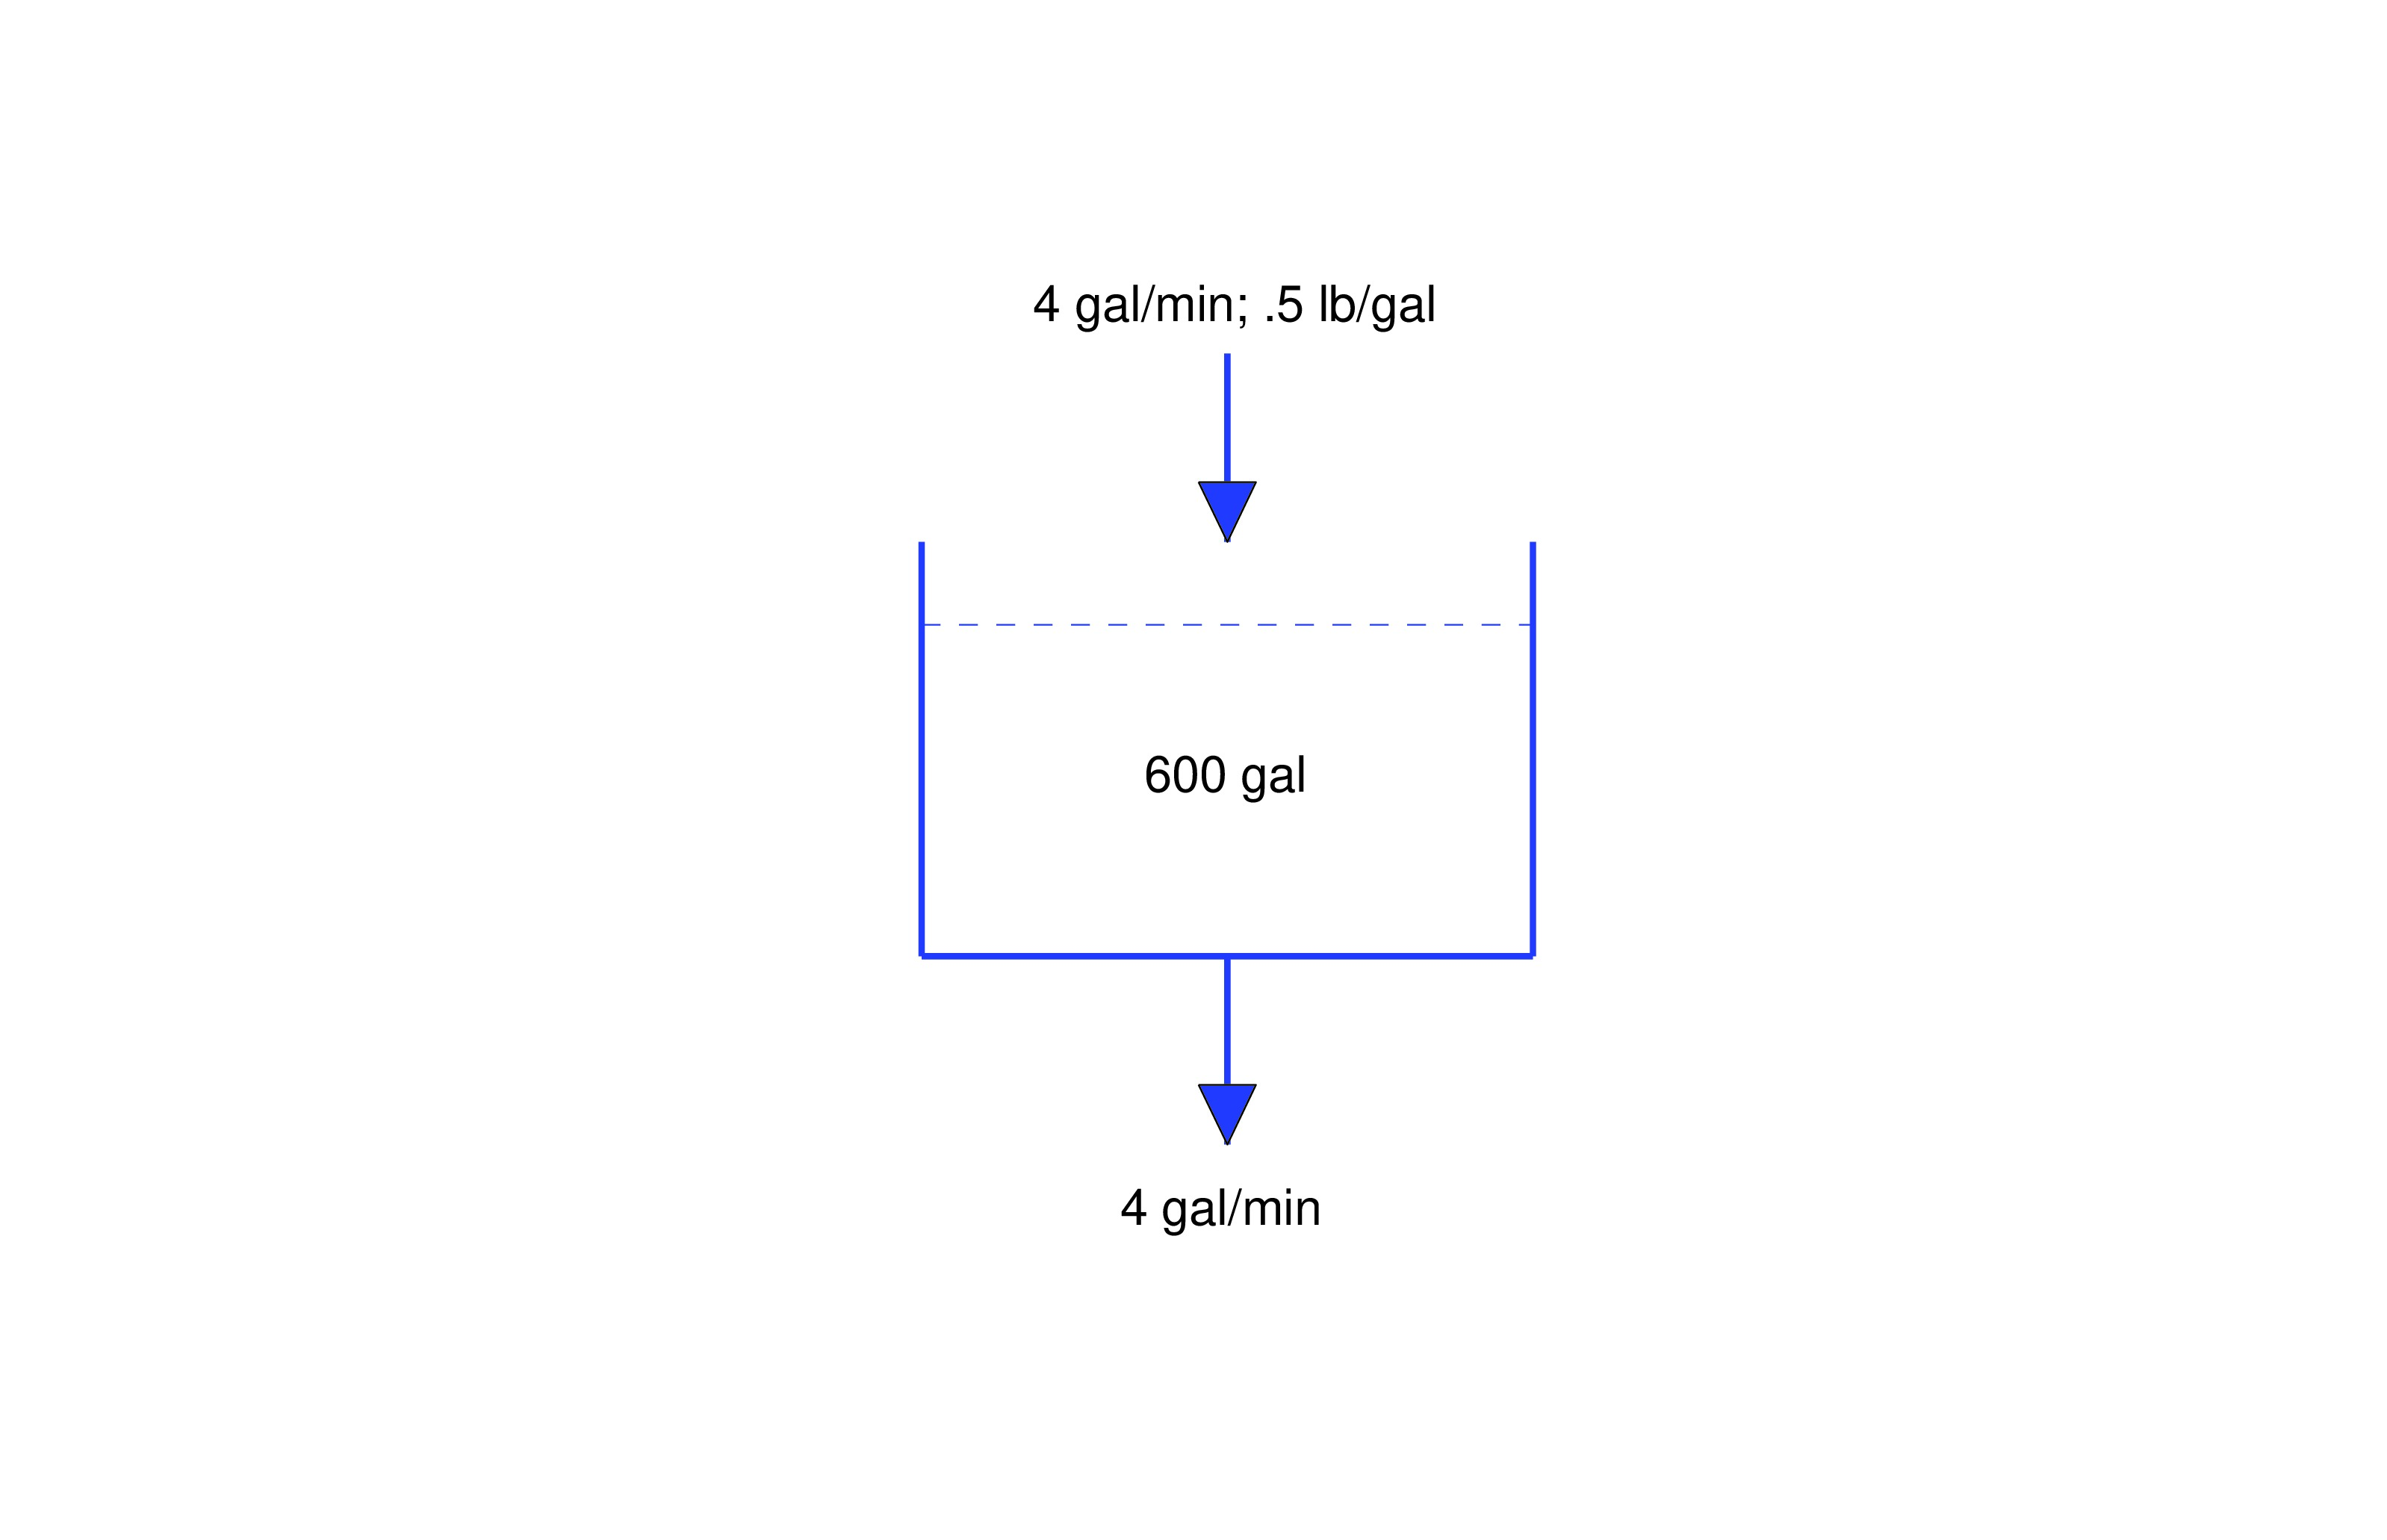
\includegraphics[height=1.5in]{fig040203.jpg} 
\end{image}


\begin{enumerate}
\item \label{item:4.2.3a}
Find a differential equation for the quantity $Q(t)$ of salt in the
tank at time $t > 0$, and solve the equation to determine $Q(t)$.
\item \label{item:4.2.3b}
 Find $\lim_{t\rightarrow\infty}Q(t)$.
\end{enumerate}


\begin{explanation} \ref{item:4.2.3a} To find a differential equation for $Q$, we must use
the given information to derive an expression for $Q'$. But $Q'$
is the rate of change of the quantity of salt in the tank changes with
respect to time;
  thus, if \textit{rate in} denotes the rate at which
salt enters
the tank and \textit{rate out} denotes the rate by which it
leaves, then
\begin{equation} \label{eq:4.2.5}
Q' = \mbox{rate in}-\mbox{rate out}.
\end{equation}
The rate in is
$$
\left(\frac{1}{2}\  \mbox{lb/gal}\right) \times (4\  \mbox{gal/min}) = 2\
\mbox{lb/min}.
$$
Determining the rate out requires a little more thought. We're
removing $4$ gallons of the mixture per minute, and there are always $600$
gallons in the tank; that is, we're removing $1/150$ of the mixture
per minute. Since the salt is evenly distributed in the mixture, we
are also removing $1/150$ of the salt per minute. Therefore, if there
are $Q(t)$ pounds of salt in the tank at time $t$, the rate out
at any time $t$ is $Q(t)/150$. Alternatively, we can arrive at this
conclusion by arguing that
$$
\begin{array}{lcl}
\mbox{rate out} & = & (\mbox{concentration})\times(\mbox{rate of
flow out})\\ \mbox{}&=&(\mbox{lb/gal})\times(\mbox{gal/min})\\
&=&\frac{Q(t)}{600}\times
4=\frac{Q(t)}{150}
\end{array}
$$
 We can now
write \eqref{eq:4.2.5} as
$$
Q' = 2-\frac{Q}{150}.
$$
This first order equation can be rewritten as
$$
Q'+\frac{Q}{150} = 2.
$$
Since $e^{-t/150}$ is a solution of the complementary equation, the
solutions of this equation are of the form  $Q=ue^{-t/150}$, where
$u'e^{-t/150}=2$, so $u'=2e^{t/150}$. Hence,
$$
u = 300e^{t/150}+c,
$$
 so
\begin{equation} \label{eq:4.2.6}
Q=ue^{-t/150}=300+ce^{-t/150}
\end{equation}
See the graph of $Q$ in the figure below.

\begin{image}
  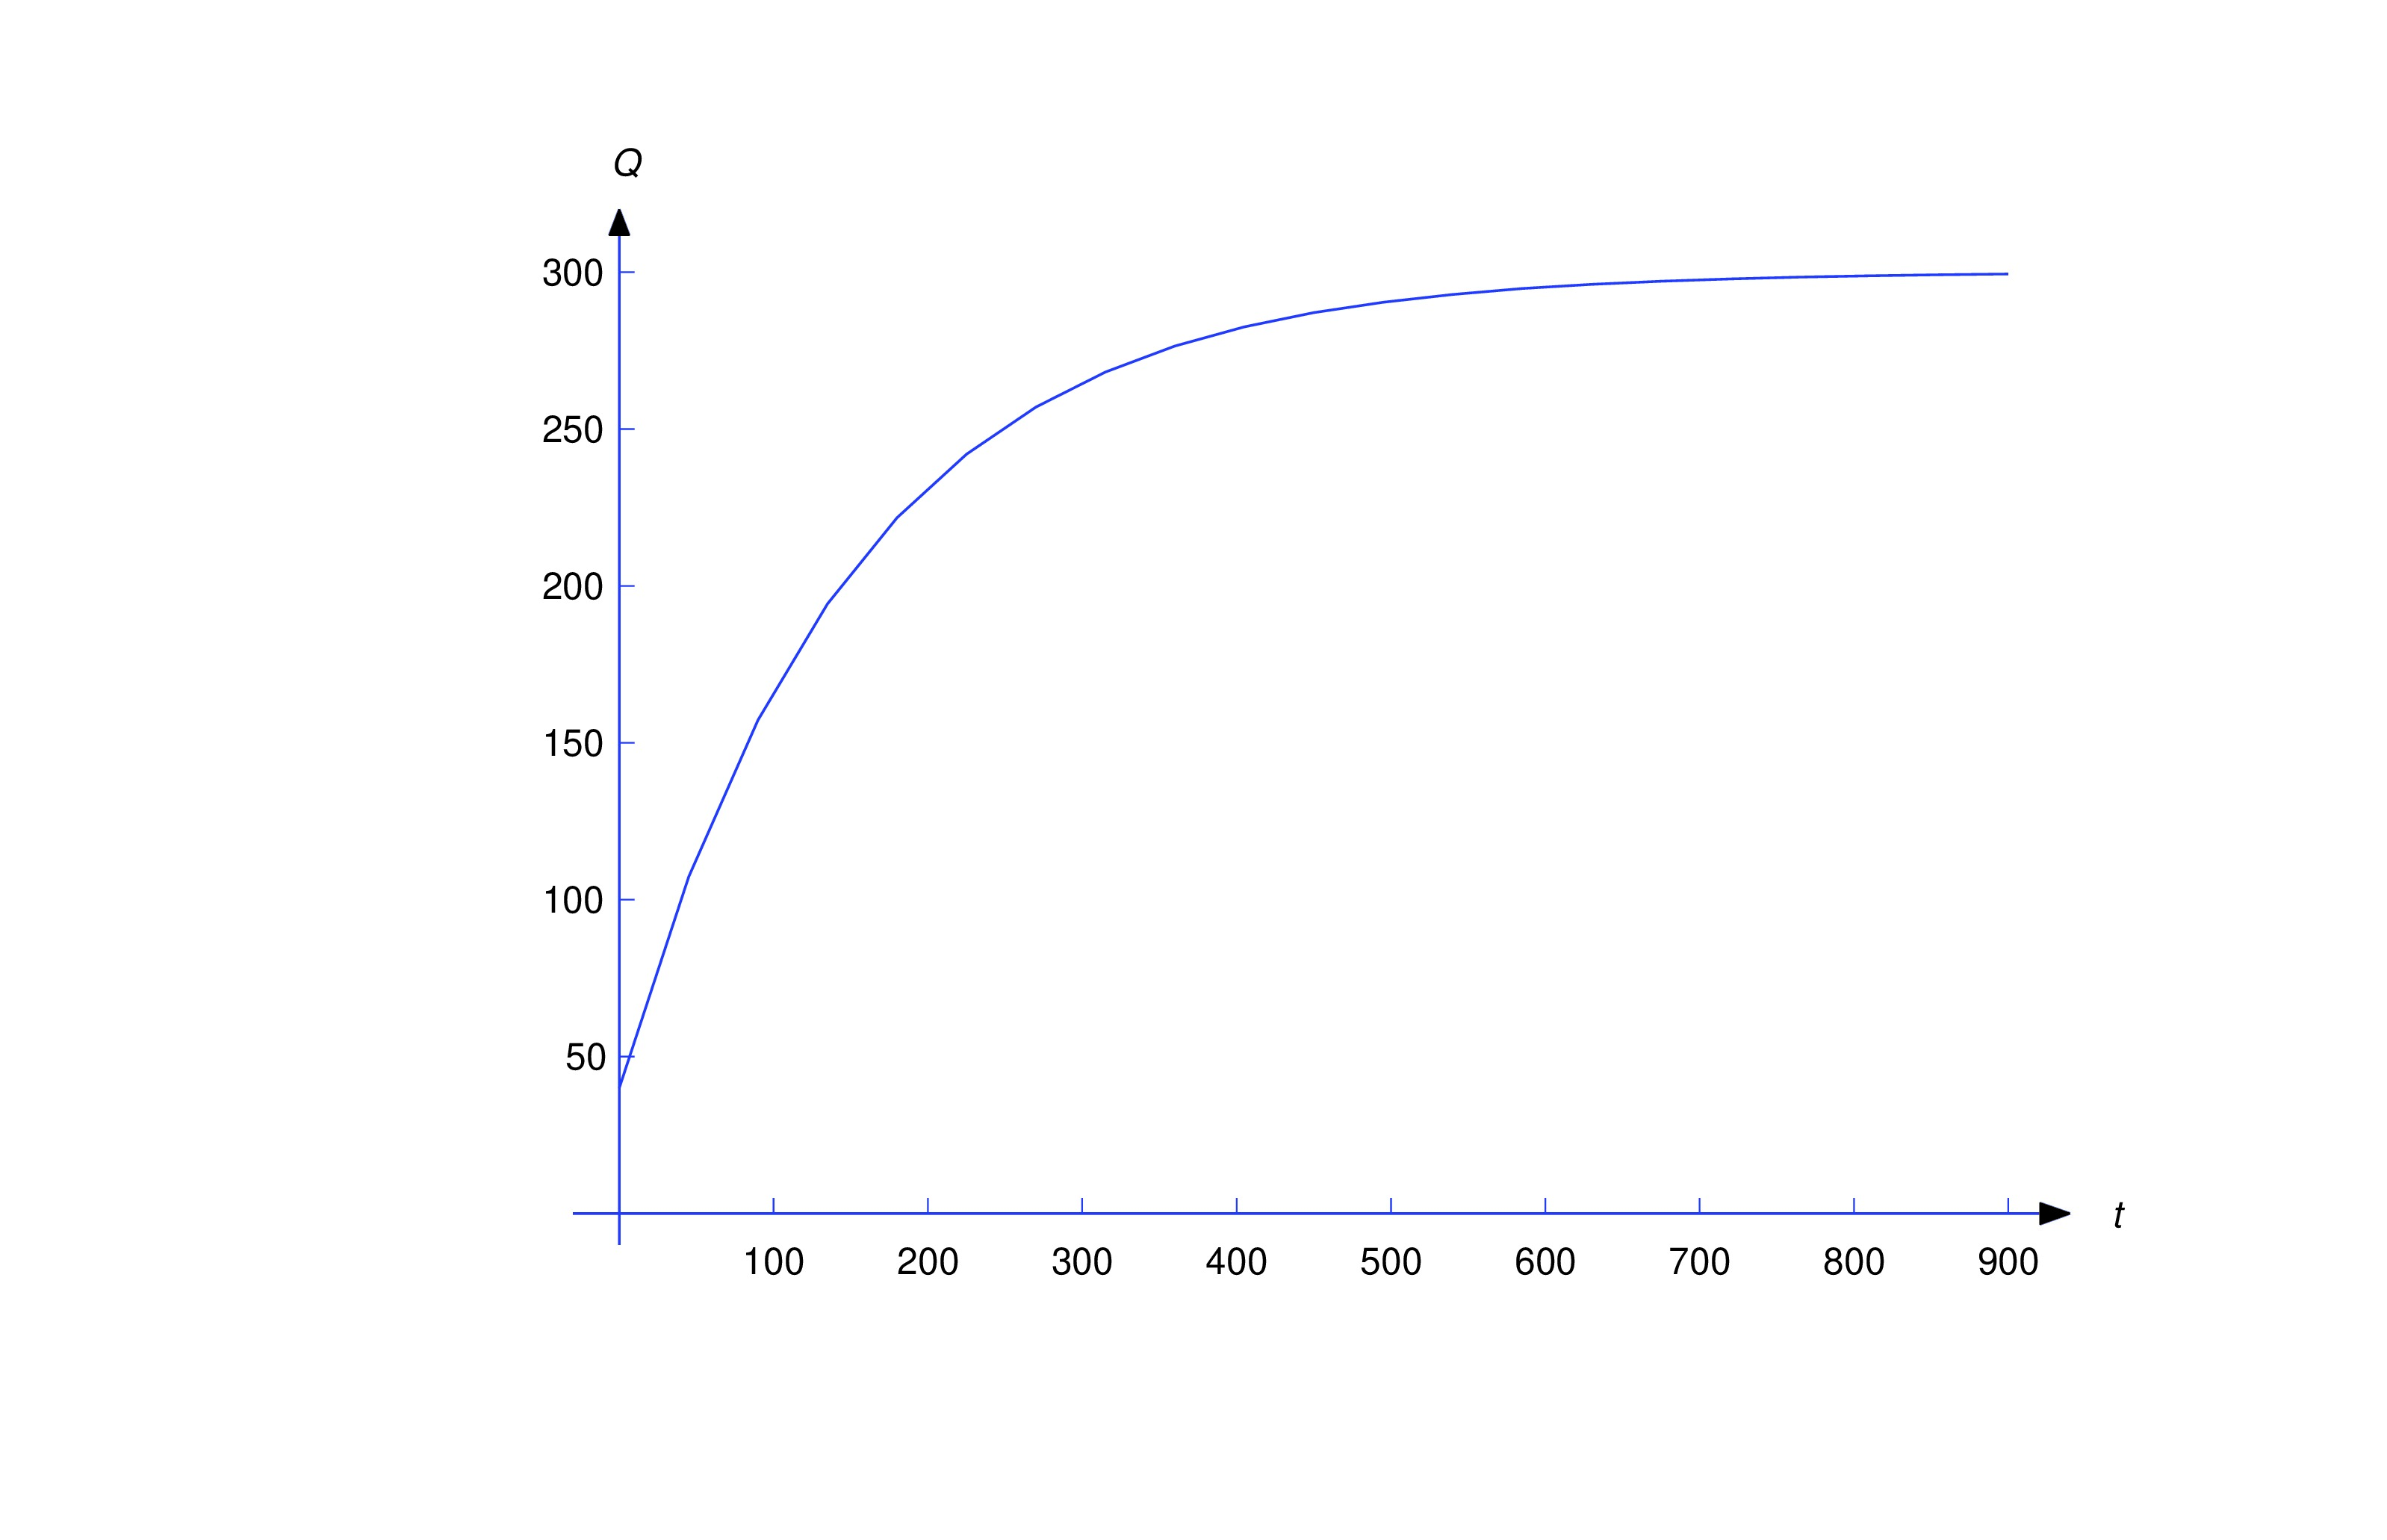
\includegraphics[height=1.5in]{fig040204.jpg} 
\end{image}

 Since $Q(0)=40$,  $c=-260$;  therefore,
$$
Q=300-260e^{-t/150}.
$$


\ref{item:4.2.3b} From \eqref{eq:4.2.6}, we see that that $\lim_{t \rightarrow
\infty}Q(t)=300$ for any value of  $Q(0)$. This is
intuitively reasonable, since the incoming solution contains $1/2$
pound of salt per gallon and there are always 600 gallons of water in
the tank. 
\end{explanation}
\end{example}

\begin{example}\label{example:4.2.4}
A $500$-liter tank initially contains $10$ g of salt dissolved in $200$
liters of water. Starting at $t_0=0$, water that contains $1/4$ g of salt
per liter is poured into the tank at the rate of $4$ liters/min and the
mixture is drained from the tank at the rate of $2$ liters/min, as shown in the figure below. 

\begin{image}
  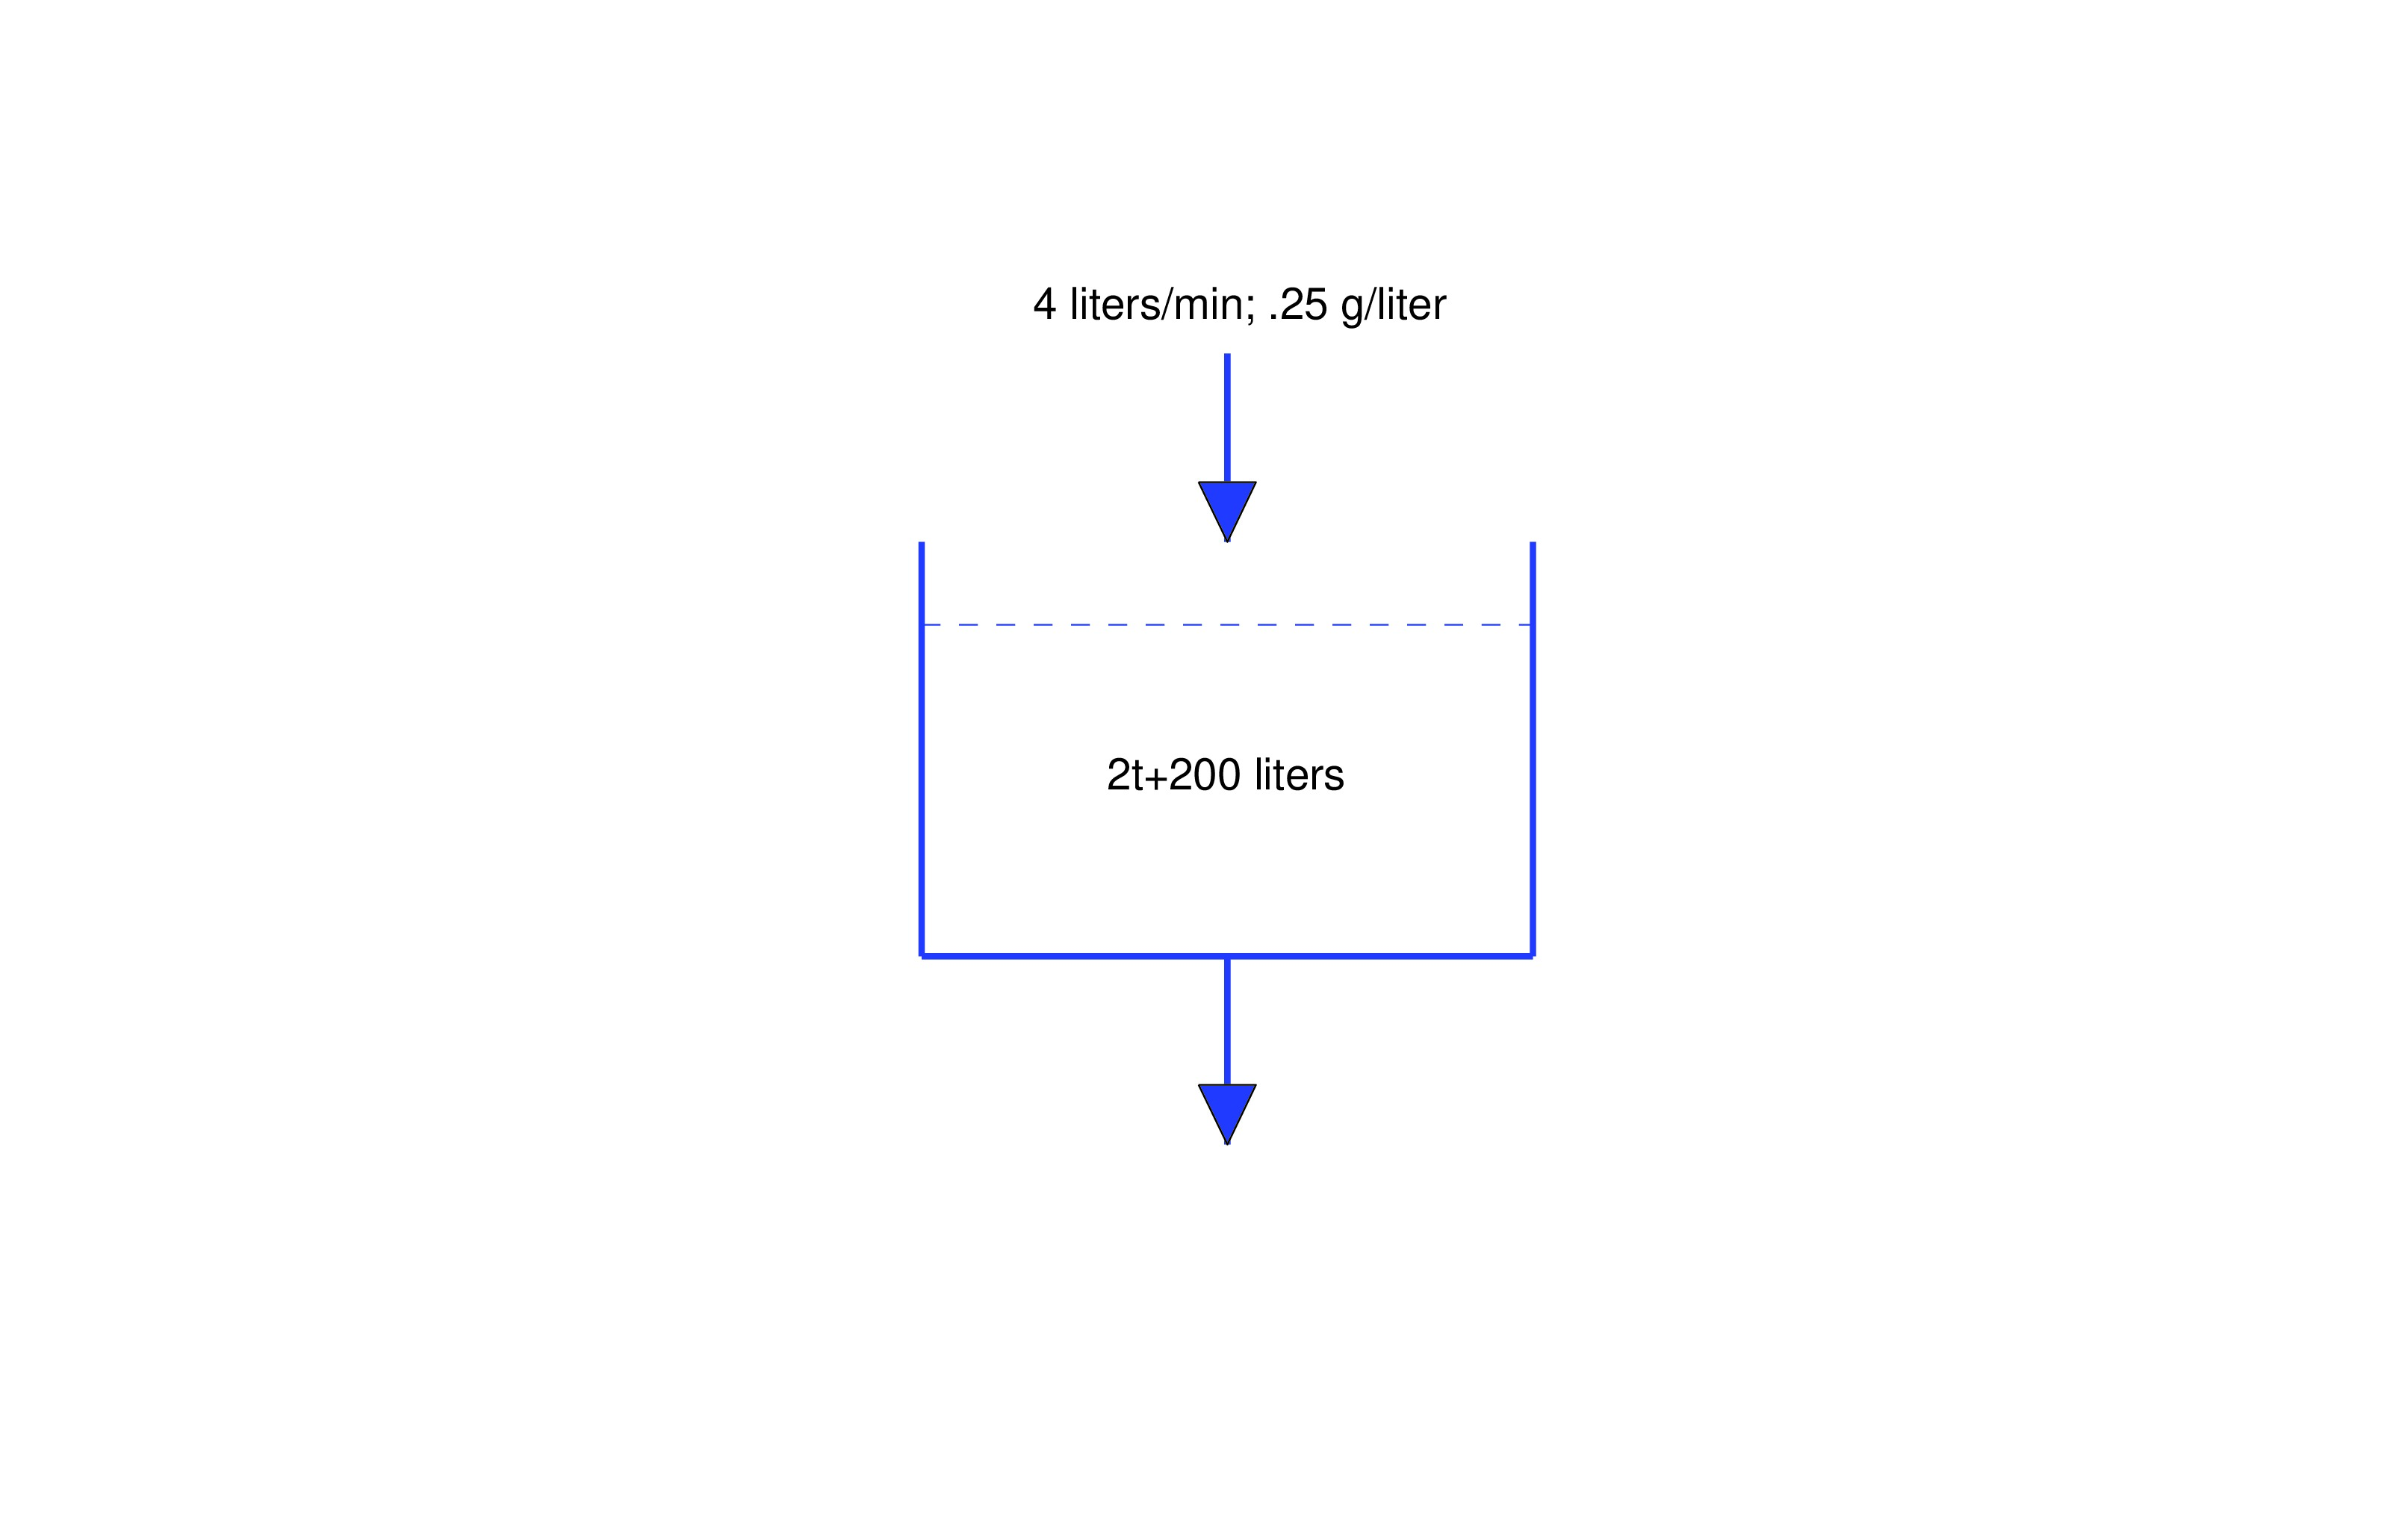
\includegraphics[height=1.5in]{fig040205.jpg} 
\end{image}

When will the tank overflow? $t=\answer{150}$ minutes.

Find a differential equation for the quantity $Q(t)$ of salt in the tank at
time $t$ prior to the time when the tank overflows and find the
concentration $K(t)$ (g/liter ) of salt in the tank at any such time.


%\begin{explanation}  
We first determine the
amount $W(t)$ of solution in the tank at any time $t$ prior to
overflow.  Since $W(0) = 200$ and we're adding $4$ liters/min while
 removing only $2$ liters/min, there's a net gain
of $2$ liters/min in the tank;  therefore,
$$
W(t) = 2t+200.
$$
 Since $W(150)=500$ liters (capacity of the
tank), this formula is valid for $0 \leq t \leq 150$.

Now let $Q(t)$ be the number of grams of salt in the tank
at time $t$, where  $0 \leq t \leq 150$.  As in Example~\ref{example:4.2.3},
\begin{equation} \label{eq:4.2.7}
Q' = \mbox{rate in}-\mbox{rate out}.
\end{equation}
 The rate in is
\begin{equation} \label{eq:4.2.8}
\left(\frac{1}{4}\  \mbox{g/liter}\,\right) \times (4\
\mbox{liters/min}\,) = 1\  \mbox{g/min}.
\end{equation}
 To determine the rate out, we observe that since
the mixture is being removed from the tank at the constant
rate of $2$ liters/min and there are $2t+200$
liters in the tank at time $t$, the fraction of the mixture
being removed per minute at time $t$ is
$$
\frac{2}{2t+200} = \frac{1}{t+100}.
$$
We're removing this same fraction of the salt per
minute.  Therefore, since there are $Q(t)$ grams of salt in
the tank at time $t$,
\begin{equation} \label{eq:4.2.9}
\mbox{rate out} = \frac{Q(t)}{t+100}.
\end{equation}
Alternatively, we can arrive at this conclusion by arguing that
$$
\begin{array}{lcl}
\mbox{rate out} & = & (\mbox{concentration})\times(\mbox{rate of
flow out})
=(\mbox{g/liter})\times(\mbox{liters/min})\\
&=&\frac{Q(t)}{2t+200}\times
2=\frac{Q(t)}{t+100}.
\end{array}
$$
 Substituting \eqref{eq:4.2.8} and \eqref{eq:4.2.9} into \eqref{eq:4.2.7}
yields
\begin{equation} \label{eq:4.2.10}
Q'=1-\frac{Q}{t+100},\quad\text{ so }\quad
Q'+\frac{1}{t+100} Q=1.
\end{equation}
By separation of variables, $1/(t+100)$ is a solution of the
complementary equation, so the solutions of \eqref{eq:4.2.10}
are of the form
$$
Q=\frac{u}{t+100},\quad\mbox{where}\quad\frac{u'}{t+100}=1,\quad\mbox{so}\quad u'=t+100.
$$
Hence,
\begin{equation} \label{eq:4.2.11}
u = \frac{(t+100)^2}{2}+c.
\end{equation}
Since $Q(0)=10$  and $u=(t+100)Q$, \eqref{eq:4.2.11} implies that
$$
(100)(10) = \frac{(100)^2}{2}+c,
$$
so
$$
c=100(10)-\frac{(100)^2}{2} =-4000
$$
and therefore
$$
u = \frac{(t+100)^2}{2} -4000.
$$
 Hence,
 $$
Q = \frac{u}{t+200}= \frac{t+100}{2}-\frac{4000}{t+100}.
$$
Now let $K(t)$ be the concentration of salt at
time $t$.  Then
$$
K(t) = \frac{1}{4}-\frac{2000}{(t+100)^2}
$$
The graph of $K$ is shown below.
\begin{image}
  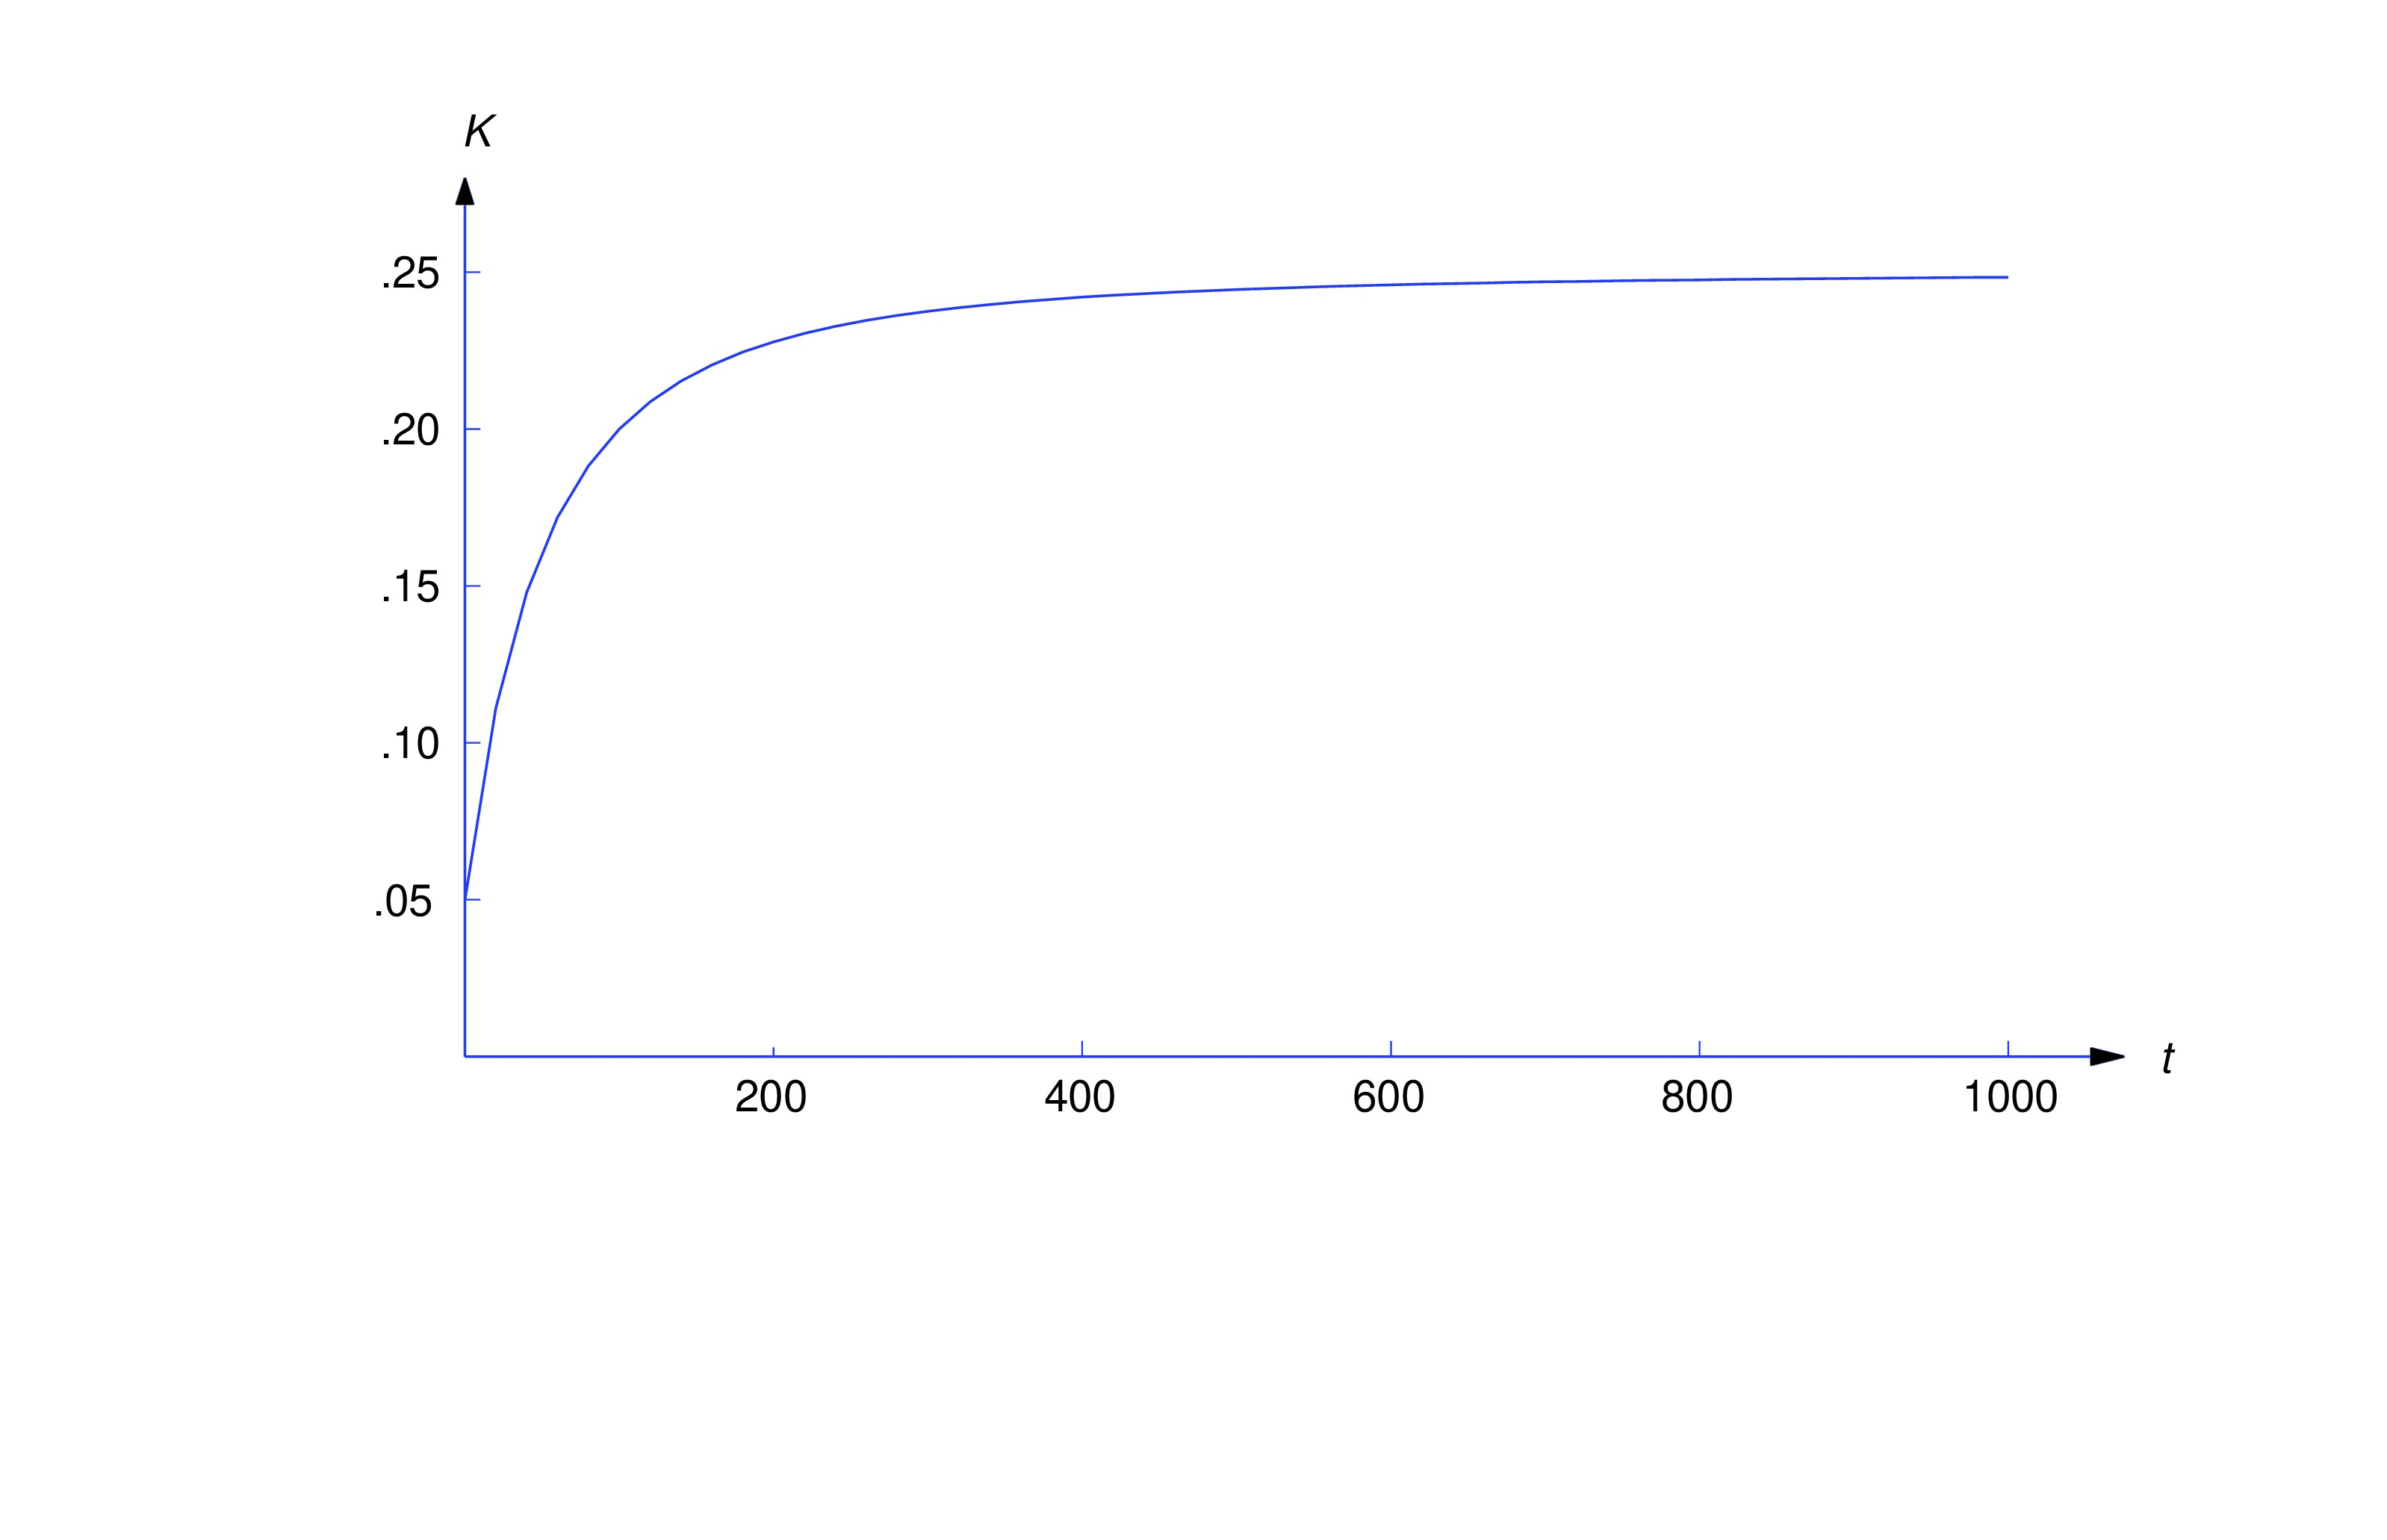
\includegraphics[height=1.5in]{fig040206.jpg} 
\end{image}

%\end{explanation}
\end{example}

\section*{Text Source}
Trench, William F., "Elementary Differential Equations" (2013). Faculty Authored and Edited Books \& CDs. 8. (CC-BY-NC-SA)

\href{https://digitalcommons.trinity.edu/mono/8/}{https://digitalcommons.trinity.edu/mono/8/}


\end{document}